\subsection{Iteration \#3}


\subsubsection*{User story}


%kommentar
\begin{figure}[H]
	\centering
	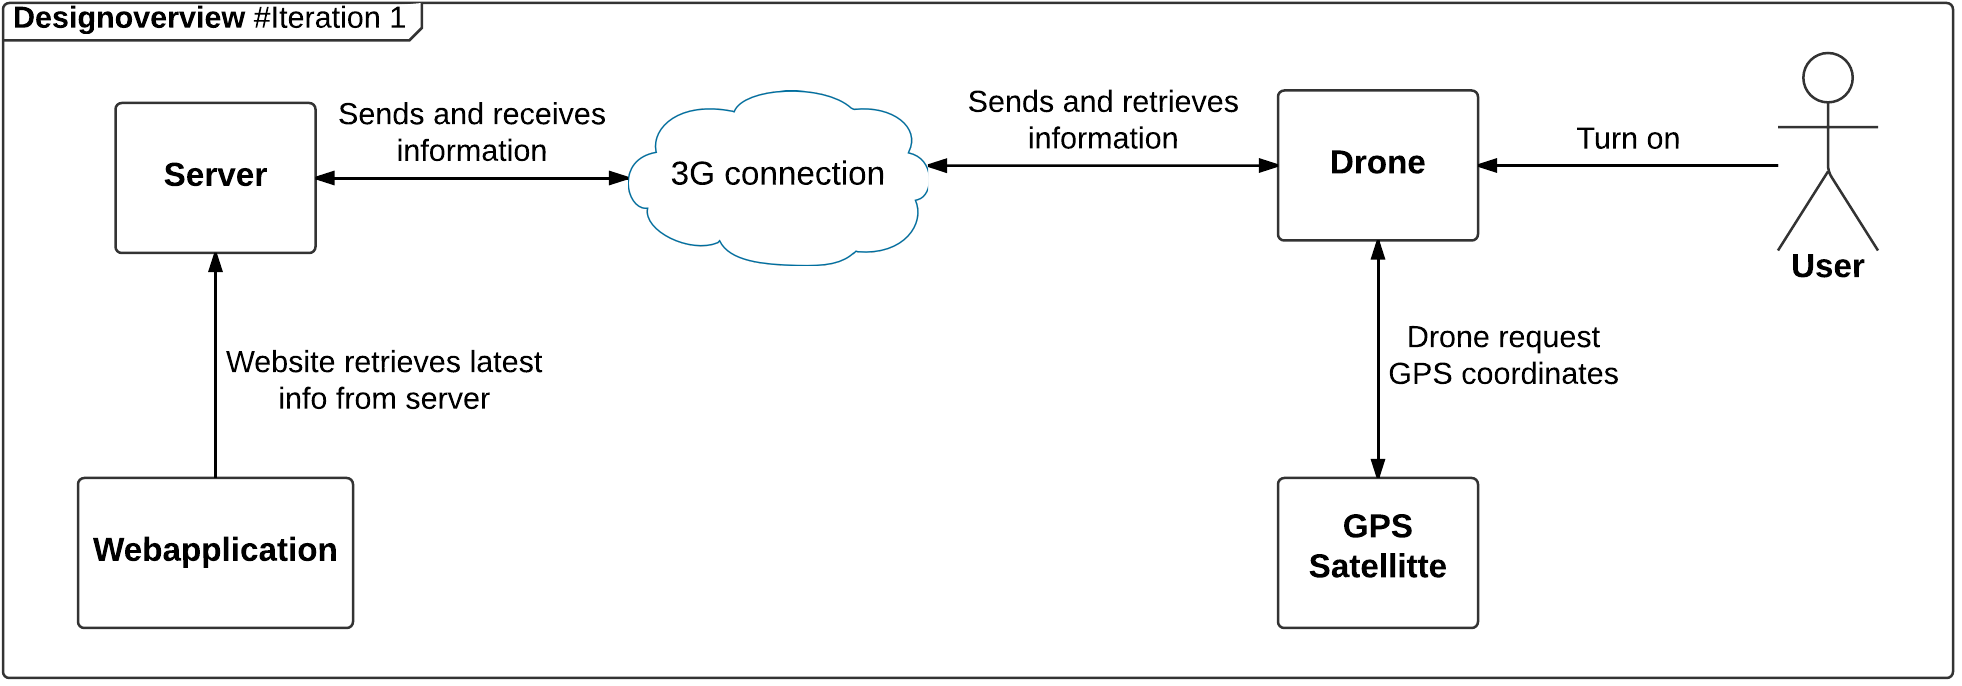
\includegraphics[width=1\textwidth]{Billeder/design_overview/design_overview_iteration1.png}
	\vspace{-.5cm}
	\caption{Design overview \#iteration 1}
	\label{fig:design_overview_UC1}
\end{figure}


\newpage
\subsubsection*{Sekvens diagram}



%kommentar
\begin{figure}[H]
	\centering
	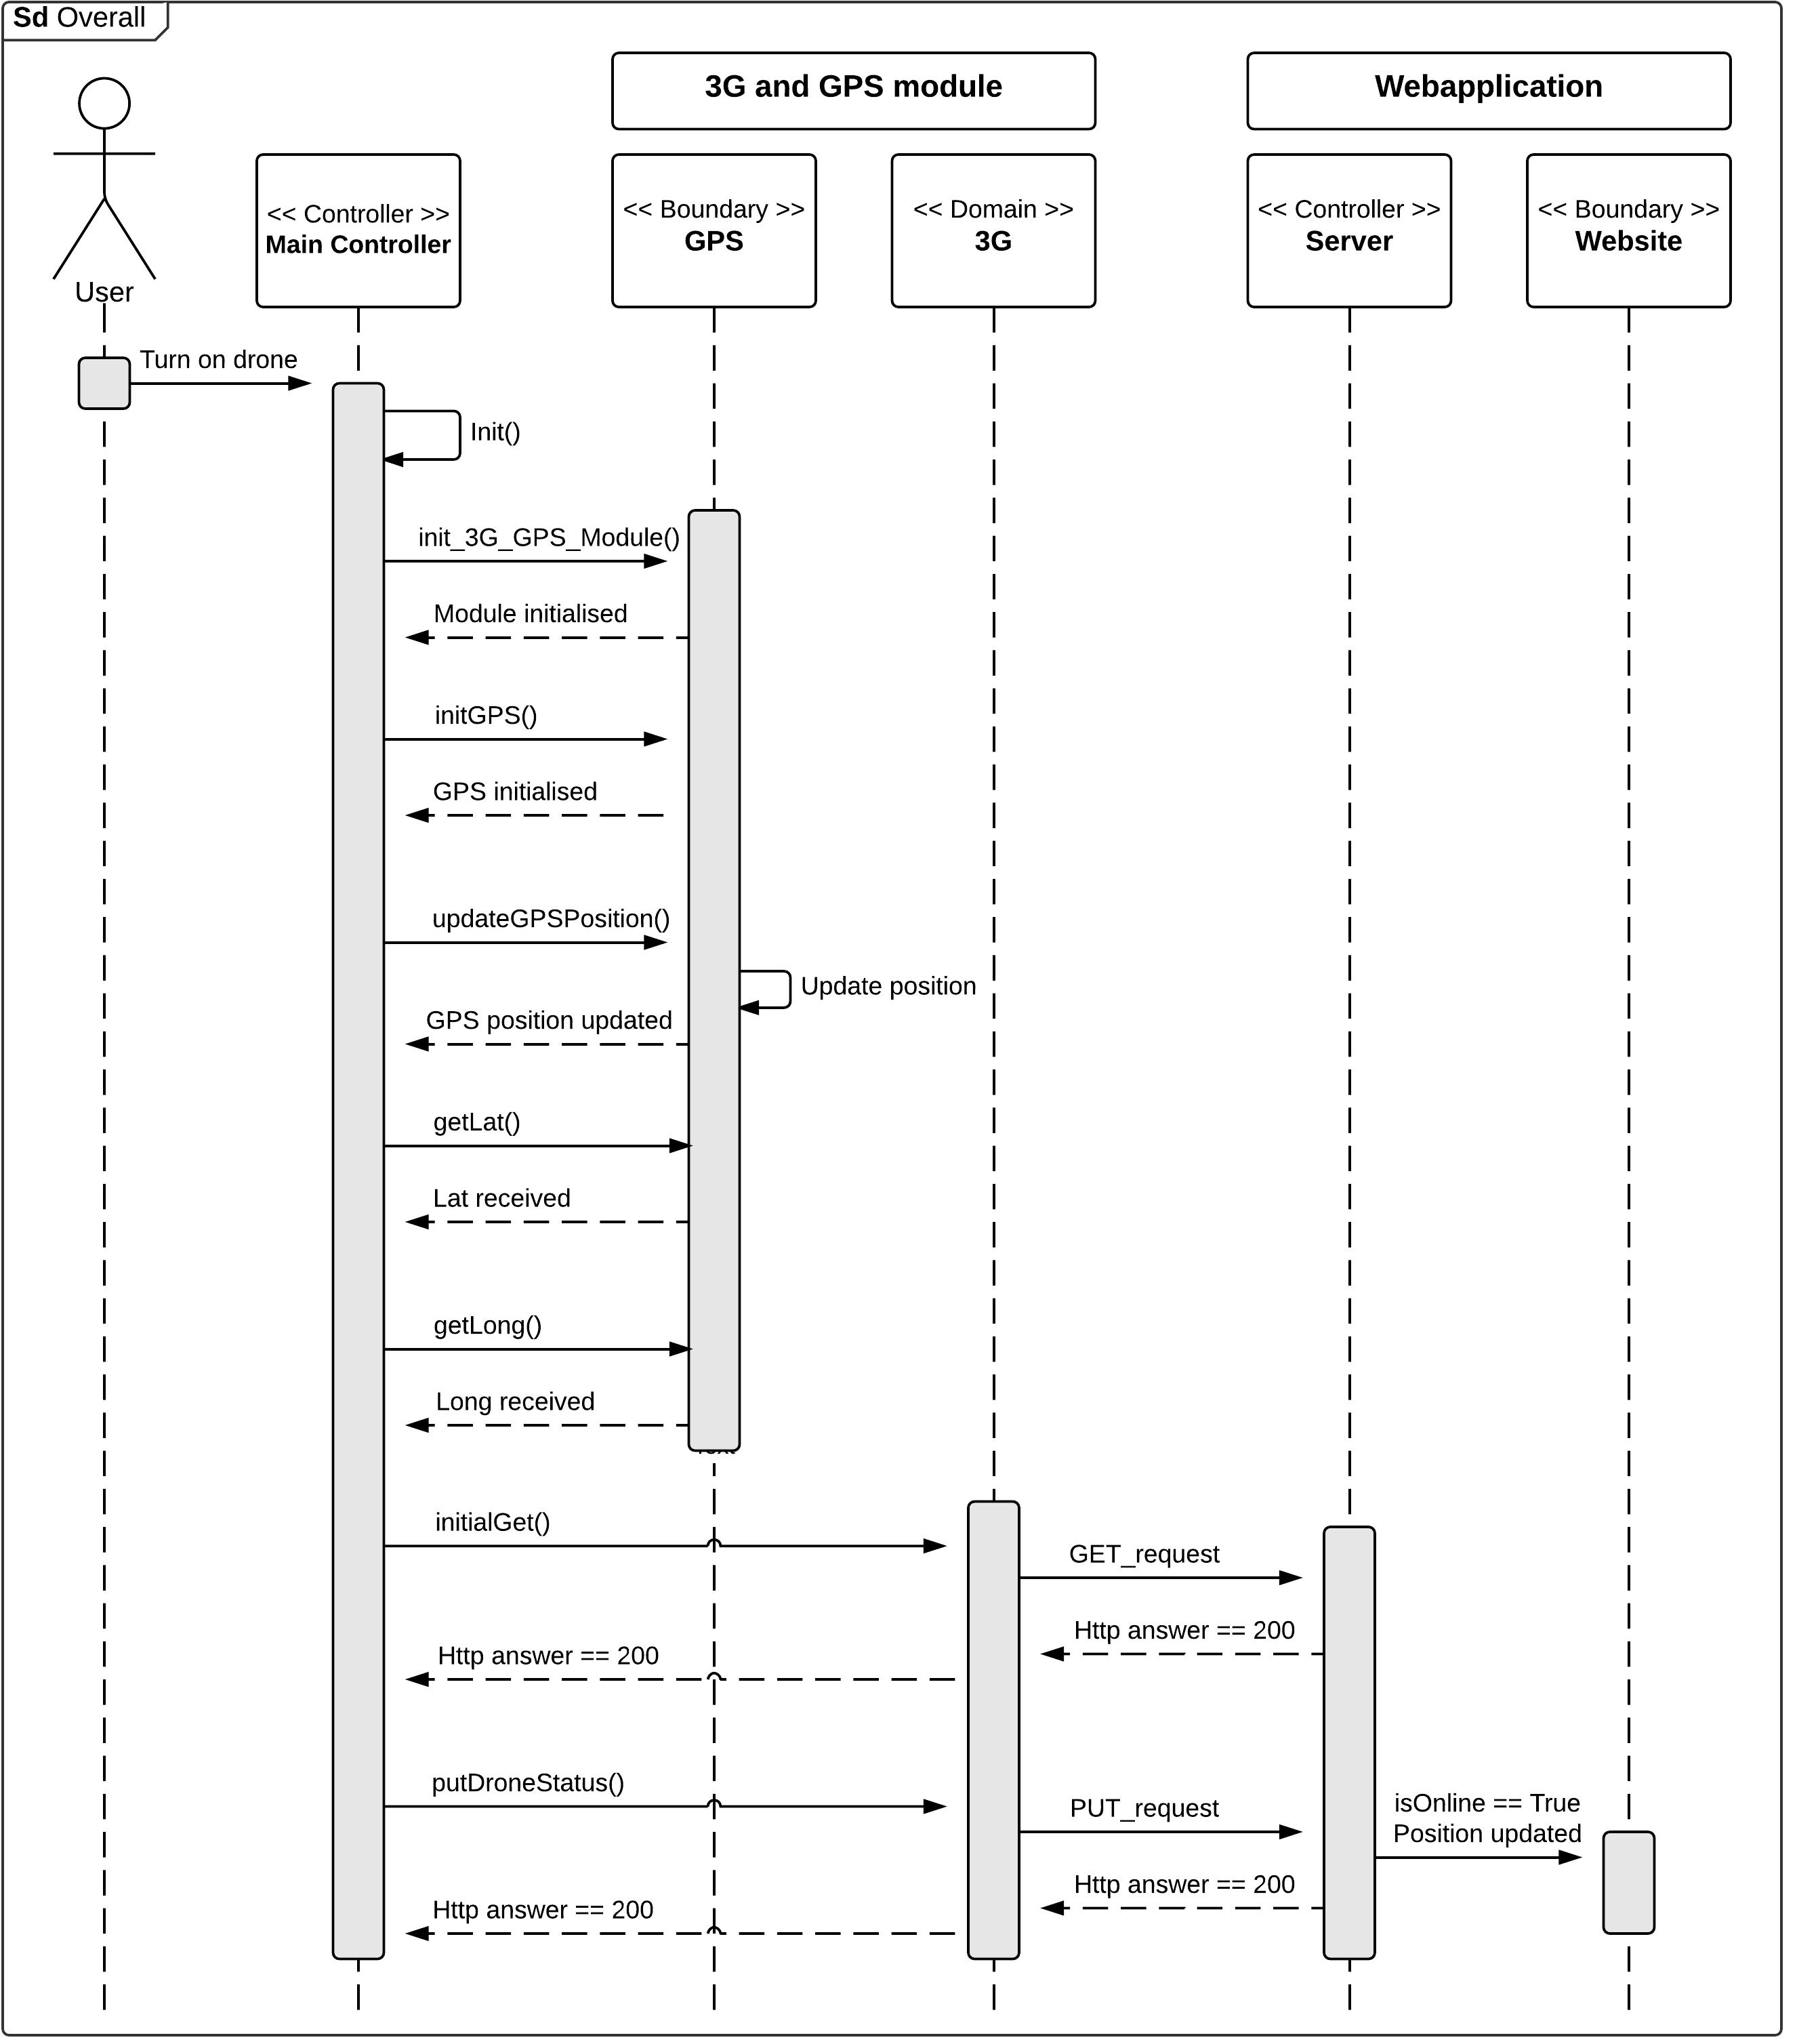
\includegraphics[width=0.93\textwidth]{Billeder/sekvens/sekvens_iteration1}
	\caption{Sekvens diagram \#iteration 1}
	\label{fig:Sekvens_diagram_iteration1}
\end{figure}
\newpage

\subsubsection*{Sekvens diagram - webapplikation}

\begin{figure}[H]
	\centering
	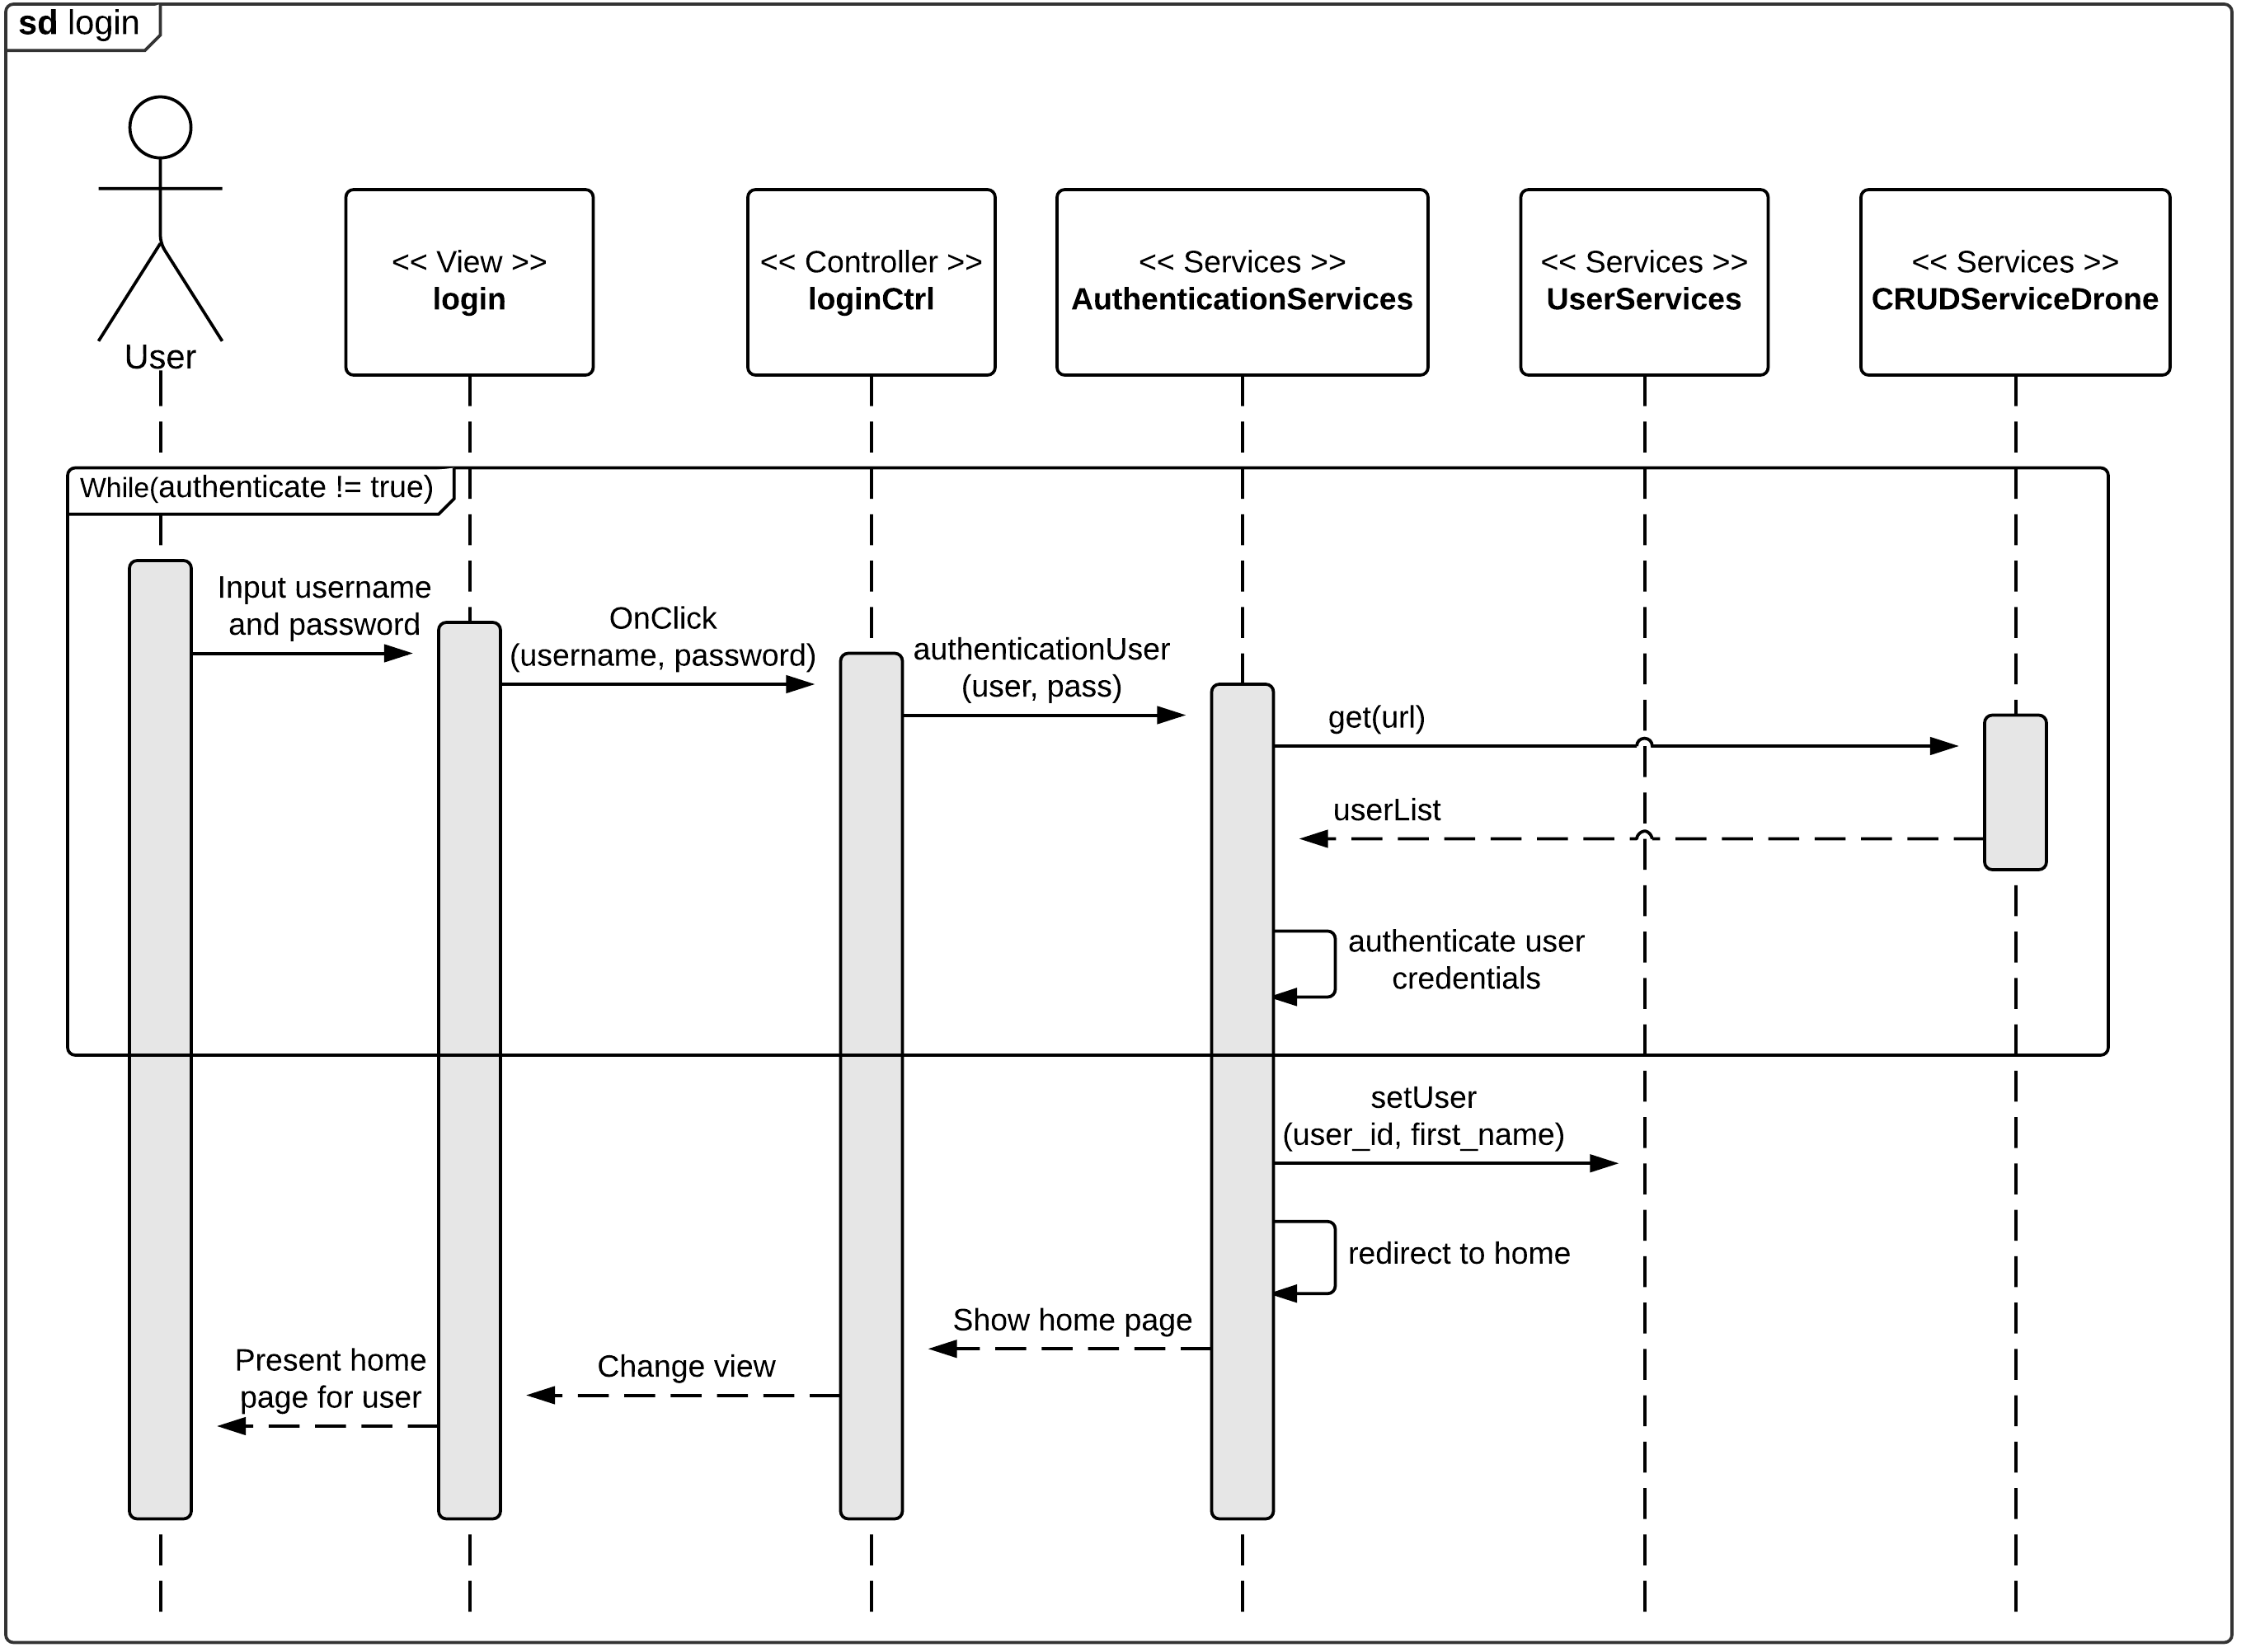
\includegraphics[width=0.93\textwidth]{Billeder/sekvens/login_sq_diagram.png}
	\caption{Sekvens diagram login}
	\label{fig:Sekvens_diagram_login}
\end{figure}
\newpage

\subsubsection*{State machine diagram}
\vspace{-0.1cm}

%kommentar
\begin{figure}[H]
	\centering
	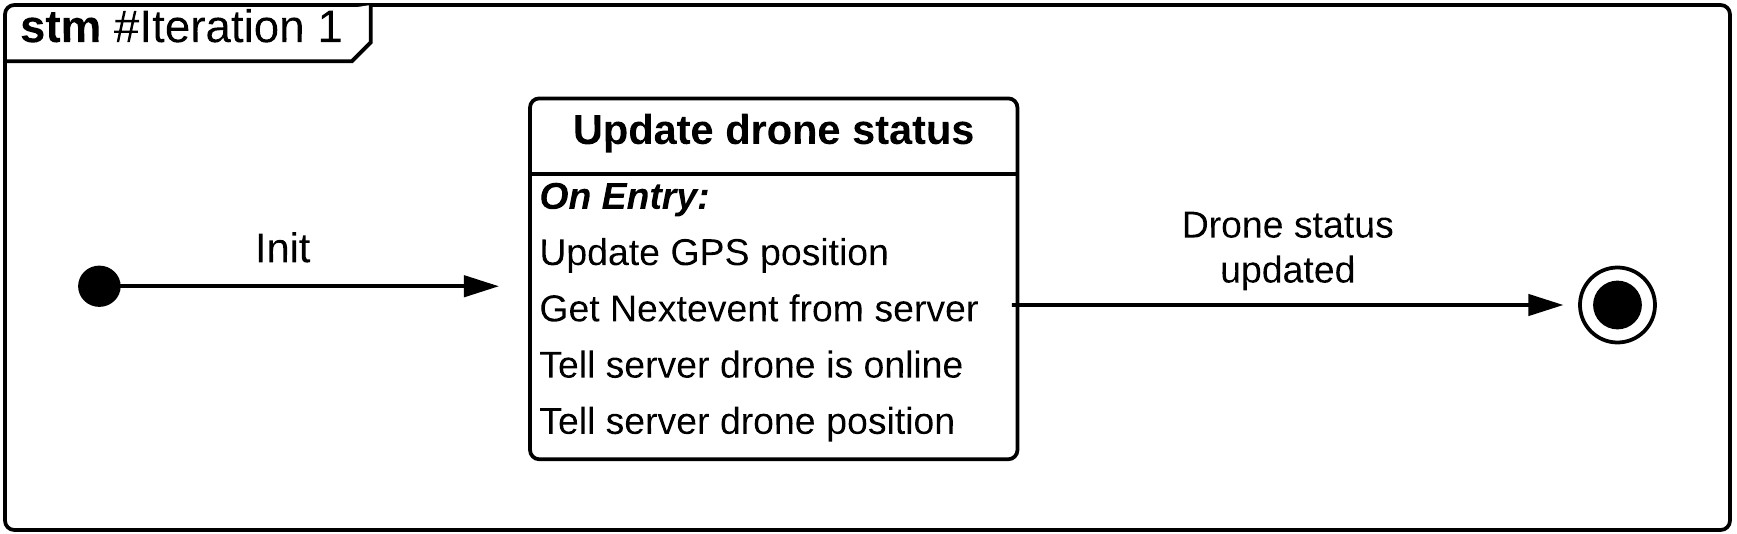
\includegraphics[width=1\textwidth]{Billeder/statemachine/State_iteration1.png}
	\vspace{-0.5cm}
	\caption{Statemachine \#iteration 1}
	\label{fig:Statemachine_iteration1}
\end{figure}
\newpage

\subsubsection*{Klasse diagram}
\vspace{-0.1cm}

%kommentar
\begin{figure}[H]
	\centering
	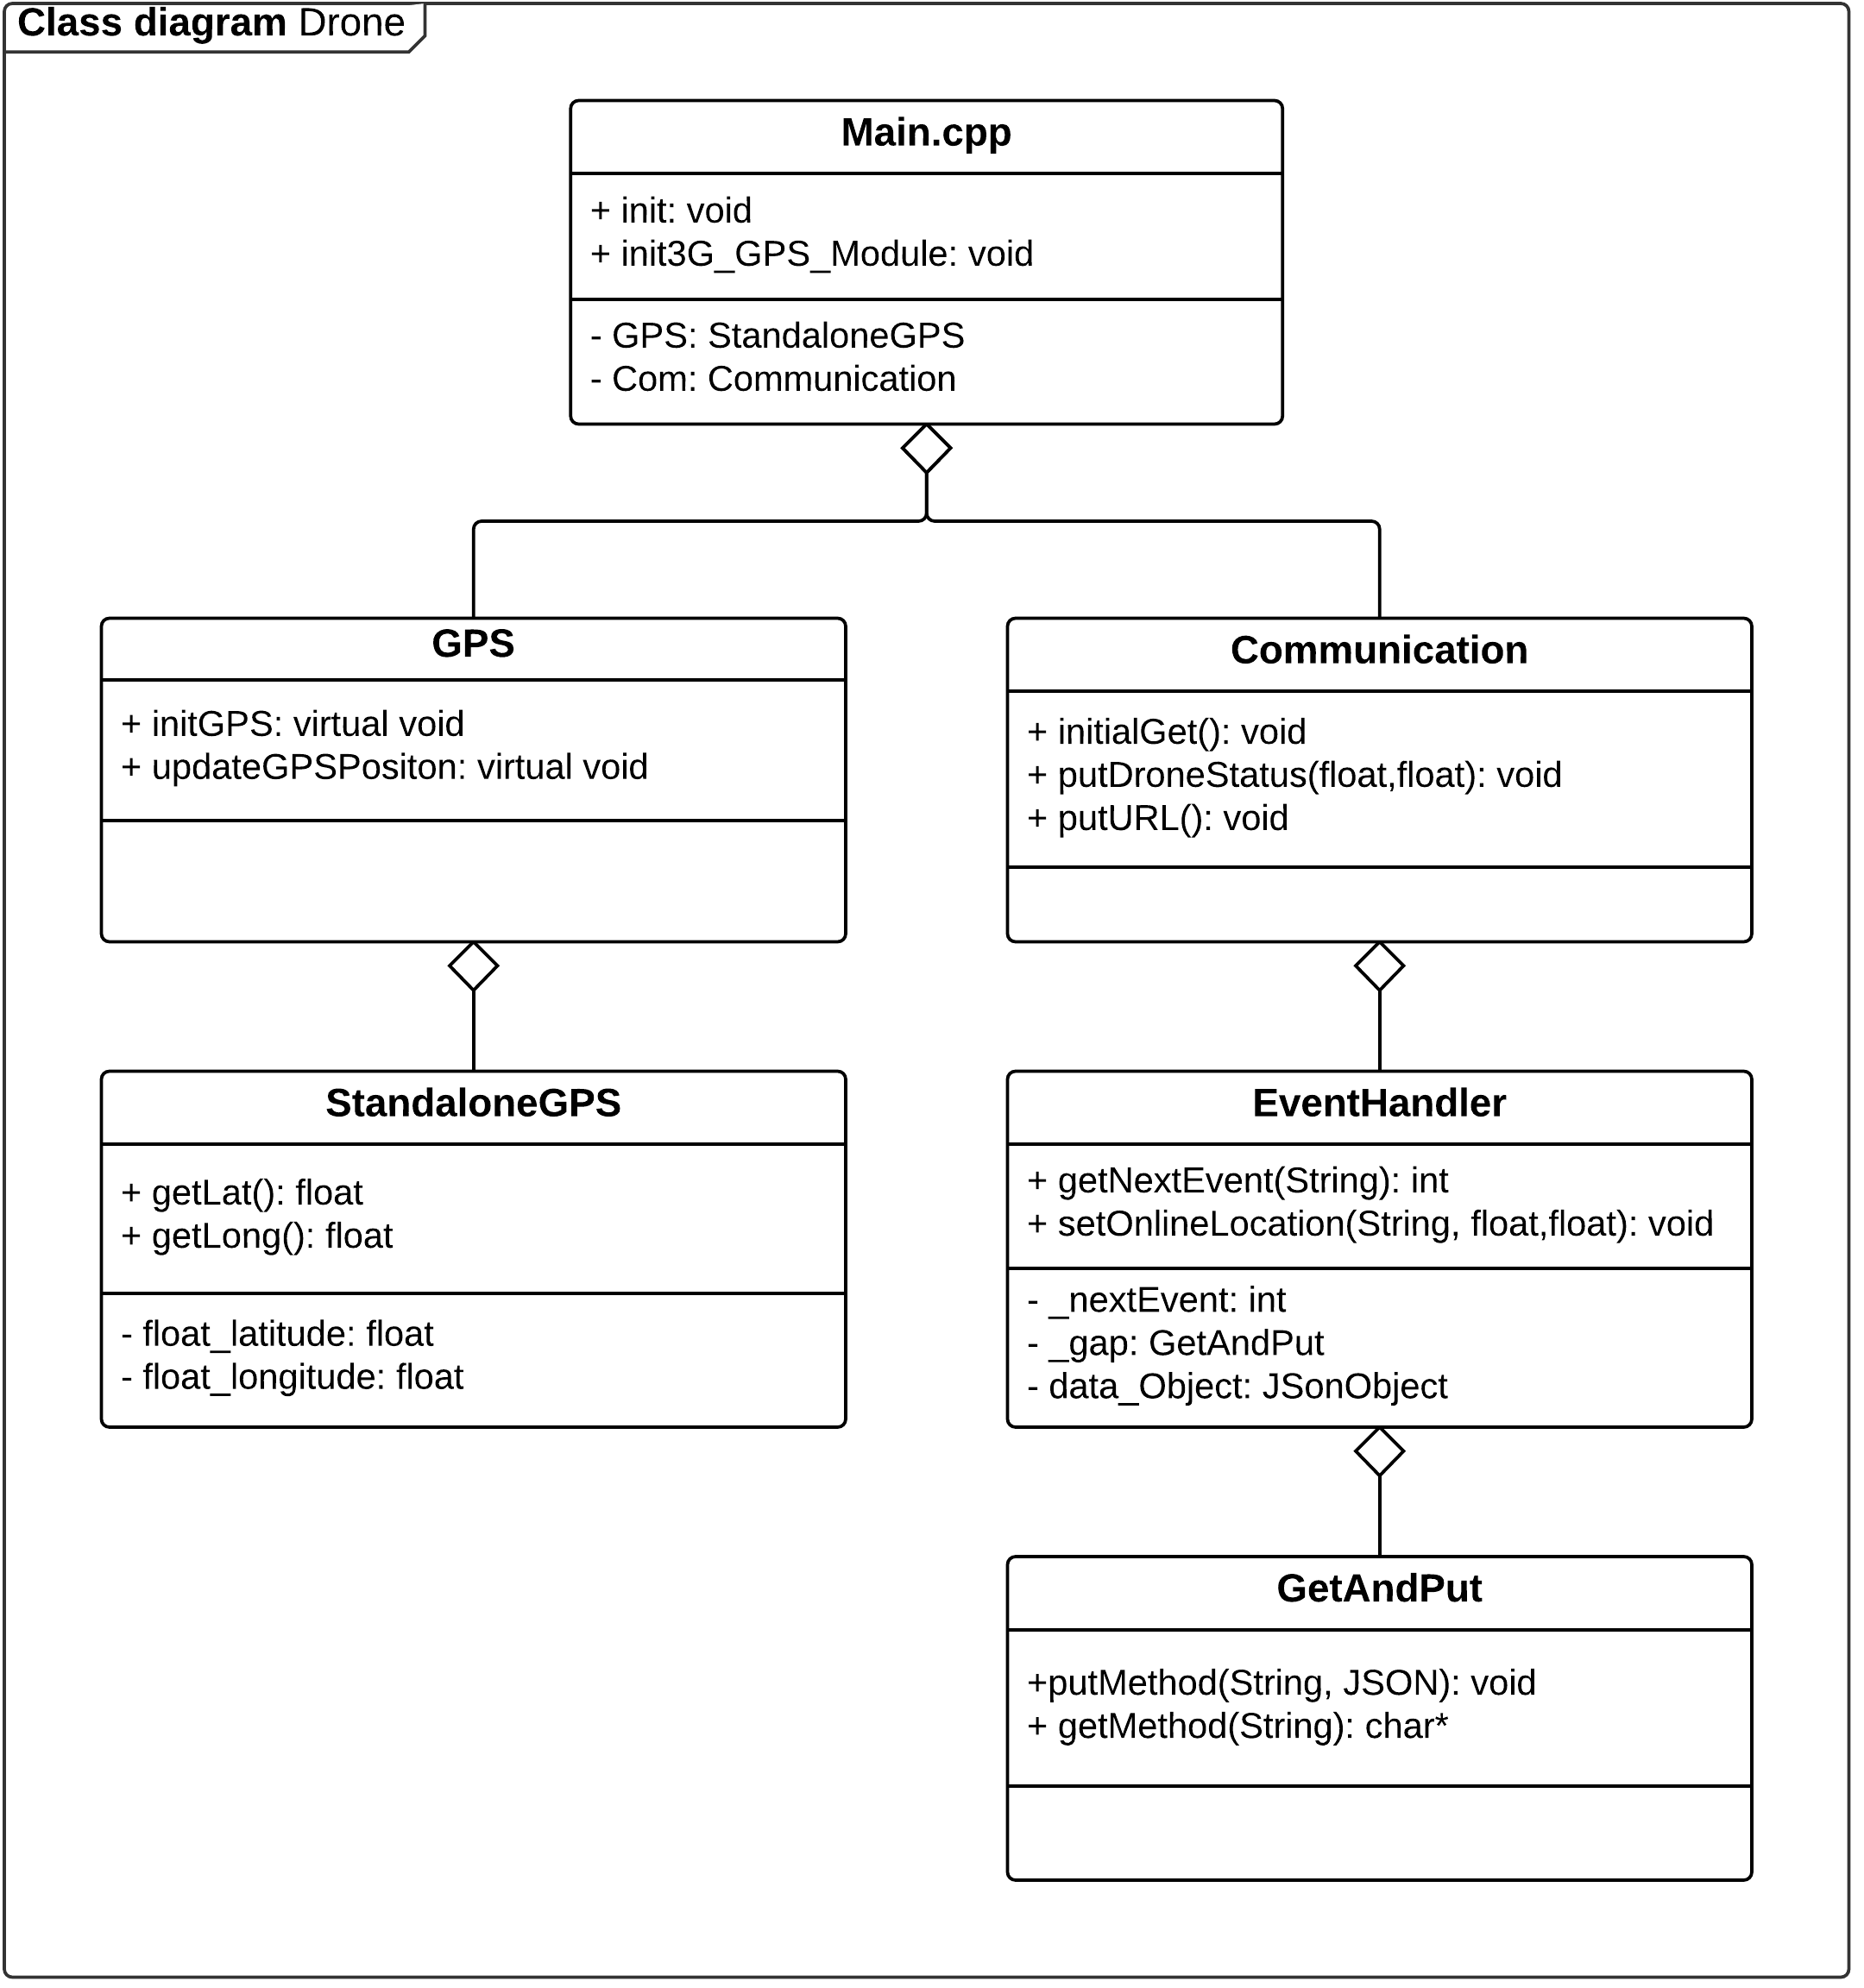
\includegraphics[width=1\textwidth]{Billeder/klasse_diagrammer/classdiagram_iteration1.png}
	\vspace{-0.5cm}
	\caption{Klassediagram \#iteration 1}
	\label{fig:classDiagram_iteration1}
\end{figure}

\newpage

\textbf{Main.cpp} \\
Main.cpp filen bruges til at sætte arduino board korrekt op, bla. sættes baudrate på de forskellige serielle forbindelser. Desuden bruges Main.cpp til at kalde og eksekverer forskellige klasse, objekter og funktioner.

\textbf{GPS} \\
GPS klassen fungerer som en virtuel klasse, og sikre som minimum implementering af init og updateGPSPosition uanset hvilken GPS der bruges. Klassen er lavet fordi der i udgangspunkt var mulighed for at bruge 3 forskellige slags GPS med 3G/GPS shieldet. 

\textbf{StandaloneGPS}\\
Denne klasse er ansvarlig for al kommunikation med GPS'en når standalone mode er valgt. 

\textbf{Module\_3G} \\
Module\_3G er ansvarlig for alt kommunikation mellem drone og server. I klassen bruges to forskellige slags http request. Når der ønskes at trække information fra sever til drone gøres der brug af GET request mens der gøres brug af PUT request når dronen ønsker at informere server om ny lokation.
